\RequirePackage{snapshot}
\documentclass[10pt,a4paper]{ULBreport}
\usepackage[utf8]{inputenc}
\sceau{Images/sceauULB.jpg}
\graphicspath{ {./Images/} }
\usepackage{multirow}
\usepackage{listings}
\usepackage{color} 
\usepackage{setspace} 
\usepackage{amsmath}

\usepackage{pdfpages}
\usepackage{biblatex}
\usepackage{floatrow}
\usepackage{subcaption} 
\usepackage{siunitx}
\usepackage[many]{tcolorbox}
\usepackage{multirow}
\usepackage{soul}
\usepackage[final]{pdfcomment}
\usepackage{listings}
\usepackage[dvipsnames]{xcolor}
\usepackage{fancyvrb}
\usepackage{hyperref}
\usepackage{xstring}
\usepackage{etoolbox}
\usepackage{svg}

%\setcounter{chapter}{-1}

% Colors


% BOXES FOR QUESTIONS

\newtcolorbox{questionBox}[2][]{
    fontupper=\bf,
    boxrule=1.5pt,
    colframe= black, % frame color
    fonttitle=\itshape,
    attach boxed title to top left={yshift=-0.3\baselineskip-0.4pt,xshift=2mm},
    title= #2,#1,
    enhanced,
    }

\newtcolorbox{bonusQuestionBox}[2][]{
    fontupper=\bf,
    boxrule=1.5pt,
    colframe= Peach, % frame color
    colback=Apricot,
    coltitle=black,
    fonttitle=\itshape,
    attach boxed title to top left={yshift=-0.3\baselineskip-0.4pt,xshift=2mm},
    boxed title style={colback=BurntOrange},
    title= #2,#1,
    enhanced,
    }





\begin{document} 


	\titleULB{
	title={Report Lab 4 \\ Virtual Private Network (VPN)},
    studies={IRELE - MA1 Electrical Engineering},
    course ={ELEC-H417},
    author={\textit{Authors :} \\ Amaury ARICO \\ Alexis BOLLENGIER \\ Emmeran COLOT \\Sefa GÖNEN  },
    date={\textbf{Academic year :} \\ 2024 - 2025},
    teacher={\textit{Professor : } \\ Jean-Michel DRICOT \\\textit{Assistant : } \\ Navid LADNER },
    logo={Images/logo-polytech.jpg},
    manyAuthor
	}

\chapter{Mission 1 - Clear traffic observation}

\begin{figure}[H]
    \centering
    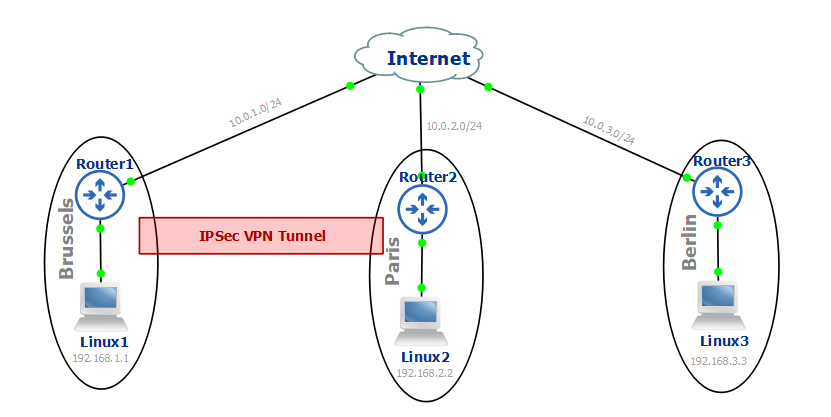
\includegraphics{Images/topology.png}
    \caption{Topology of the network for the lab}
    \label{img:topology}
\end{figure}


\section{Question - Netmask adaptation}

\begin{questionBox}{Netmask adaptation}
    What should be the netmask to achieve this and why ?
\end{questionBox}


The payload \footnote{The payload was sent from Linux1 (\textit{192.168.1.1}) to Linux2 (\textit{
192.168.2.2}) and contained "Network architecture is fun"} is at the end (\textit{layer 7} data) of the $4^{th}$ 
packet. To ensure that the message is received, 
it is sent in \textbf{TCP} and this is the reason of the number of packet sent (7) despite 
the fact that the content of the message was only 28 bytes.\\
Let's analyze each request:

\begin{enumerate}
    \item \textbf{Linux1} $\rightarrow$ \textbf{Linux2}, wanting to instantiate the connection with the \textbf{SYN} 
    flag raised (for synchronization)
    \item \textbf{Linux2} $\rightarrow$ \textbf{Linux1}, acknowledging (\textbf{ACK} flag + \textit{Ack=1}) the 
    reception of the synchronization (\textbf{SYN} flag) request
    \item \textbf{Linux1} $\rightarrow$ \textbf{Linux2}, acknowledging (\textbf{ACK} flag + \textit{Ack=1}) the 
    acknowledgment of Linux2
    \item \textbf{Linux1} $\rightarrow$ \textbf{Linux2}, pushing the payload (\textbf{PSH} flag) and still
    acknowledging the reception of the $2^{nd}$ packet (\textbf{ACK} flag + \textit{Ack=1})
    \item \textbf{Linux1} $\rightarrow$ \textbf{Linux2}, informing it of the finish of the transmission (\textbf{FIN}
    flag). It is necessary because if the payload is too long, it would have needed multiple push
    requests. This packet still acknowledges the last received packet (\textbf{ACK} flag + 
    \textit{Ack=1})
    \item \textbf{Linux2} $\rightarrow$ \textbf{Linux1}, acknowledging the reception of the $4^{th}$ packet
    (\textbf{ACK} flag + \textit{Ack=29})
    \item \textbf{Linux2} $\rightarrow$ \textbf{Linux1}, acknowledging the reception of the $5^{th}$ packet
    (\textbf{ACK} flag + \textit{Ack=30})
\end{enumerate}

To finish this analysis, let's just recall how the \textit{acknowledgment number} is determined:
when sending a packet of \textit{sequence number} $N$ and payload of length $M$, the expected acknowledgment response
number is $M + N$. This number corresponds also to the sequence number of the next packet to send.

\begin{figure}[H]
    \centering
    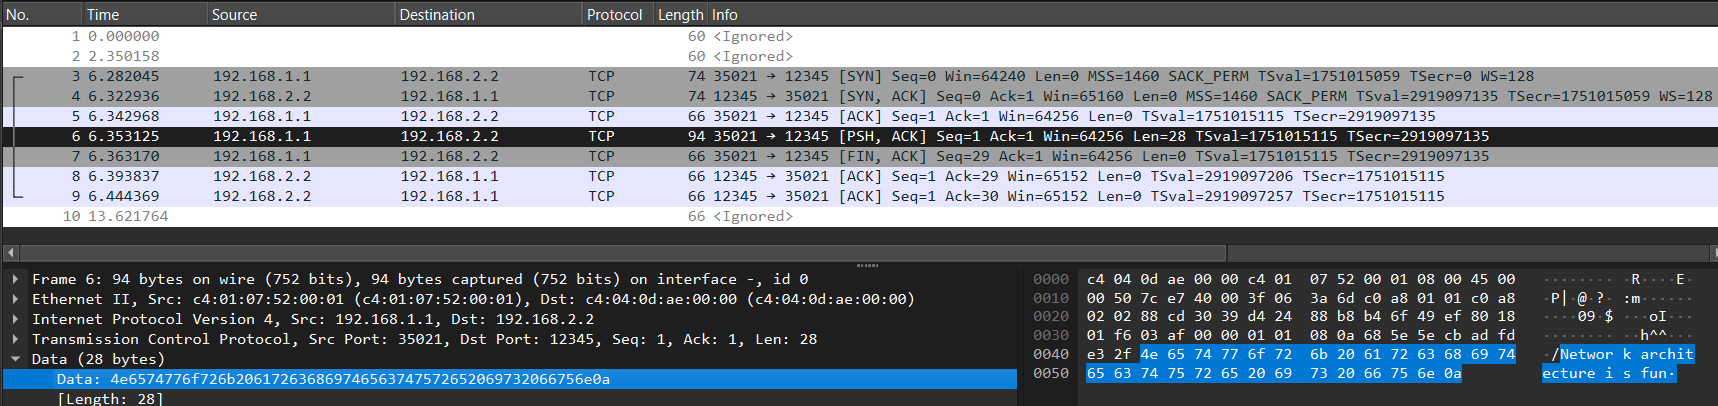
\includegraphics[width=\textwidth]{Images/wireshark0.png}
    \caption{Wireshark capture of an \textit{echo} request}
    \label{img:wireshark_1_1}
\end{figure}

\section{Bonus question - One-way communication}

\begin{bonusQuestionBox}{One-way communication}
    What can you do to make a one way communication (i.e. ping PC1→PC2 works but not PC2→PC1) ?
\end{bonusQuestionBox}


The explanation at the end of the previous question can be studied more in depth:\\
The \textbf{sequence number} is a value linked to the sender side\footnote{both PCs are senders and receivers} that indicates the packet that he is
sending. This number is in fact a pointer that is set to $0$ at the start of the communication.\\
The \textbf{acknowledgment number} is a value linked to the receiver side that indicates the next packet's sequence number that the receiver expects to receive. The calculation has been explained in the previous section (seq + length).\\
It can be seen on the Wireshark screenshot \ref{img:wireshark_1_1} that Linux1 send the packet
with sequence number $29$ without waiting for the acknowledgment number $29$ to avoid waiting
twice the travel time. In the case this acknowledgment never arrived, Linux1 would have sent
the packet with sequence number $1$ again.


\chapter{Mission 2 - VPN configuration}

\section{Question - IPv6 compatibility}

\begin{questionBox}{IPv6 compatibility}
    From PC1, ping Router1 and PC2 IPv4 and IPv6 addresses. What is working ? Why ?    
\end{questionBox}


\begin{itemize}
    \item \textbf{AES encryption:} transform the data in \textit{cyphertext} in a way that is resistant to brute-force, 
    making it unreadable for anyone intercepting it. It uses the same key for encryption and decryption and is based on 
    \textit{XORing}, substituting, shifting and mixing operations.\\
    It is here used to make sure that the data cannot be read.
    \item \textbf{SHA hash function} \textit{(or Secure Hash Algorithm)}\textbf{:} a hash function converts a message in
    a fixed-size output in a deterministic way. SHA has the particularity that even if a bit of the original data is 
    flipped, the output of the hash is entirely different.\\
    It is here used to make sure that the data has not been modified during transmission.
    \item \textbf{Pre-shared key authentication:} verifies identity using a shared secret key known by both parties. 
    This is used during the initial setup of the communication.
    \item \textbf{Group 2 Diffie-Hellman:} allows to share keys over an unsecured channel. The choice of group 2 is a
    good compromise between security and computation time.\\
    Note that it is not used to share the authentication key as it is already known by the two correspondents.
    \item \textbf{Lifetime of 86400:} Sets the duration of the security association to 24 hours. After this time, both
    parts must check the identity of the other again (for example by sending the authentication key).
\end{itemize}


\section{Question - How does Traceroute reveal the path between devices ?}

\begin{questionBox}{ How does Traceroute reveal the path between devices ?}
    By analysing carefully your trace command using Wireshark (do not hesitate to capture all the three links), you should be able to understand how it works. Explain in details how the traceroute command works (and interesting observations you can make). What are the layer 3 protocols used and why ?
\end{questionBox}


As mentioned before, it is a symmetric encryption method, meaning that the same key is used on both sides (for encryption and decryption). The benefit of it is that it is faster to decrypt/encrypt and easier to use than asymmetric encryption.

\chapter{Mission 3 - Encrypted traffic observation}



\section{Question - What is the route}

\begin{questionBox}{What is the route}
    What is the current route (IPs and devices) ? Did the route change (compared to mission 2: RIPv2) and why ?
\end{questionBox}


\begin{figure}[H]
    \centering
    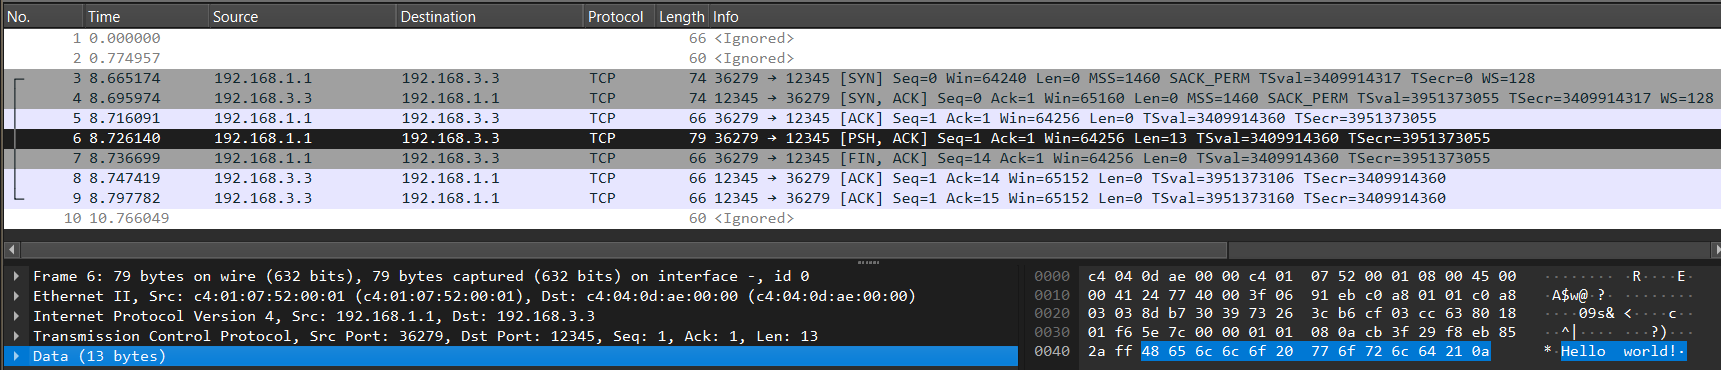
\includegraphics[width=\textwidth]{Images/wireshark2.png}
    \caption{\textbf{Berlin}: Wireshark capture of the \textit{echo} request without the VPN}
    \label{img:wireshark_2_1}
\end{figure}

\begin{figure}[H]
    \centering
    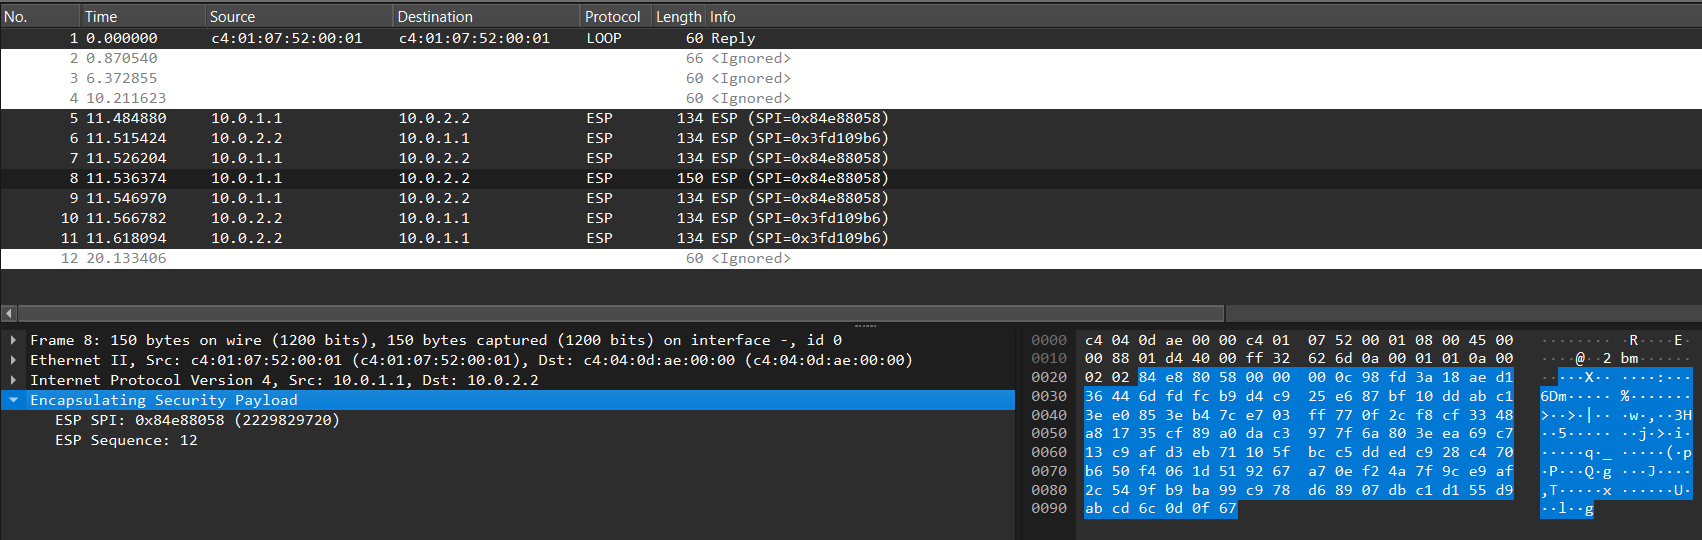
\includegraphics[width=\textwidth]{Images/wireshark1.png}
    \caption{\textbf{Paris}: Wireshark capture of the \textit{echo} request through the VPN channel}
    \label{img:wireshark_2_2}
\end{figure}

The main difference between the two situations here is that it is impossible for us
to retrieve the payload \footnote{"Hello world!"} when the payload is sent through the
VPN channel as it is encrypted. \\
Because the \textbf{IPSec} has been configured in tunnel
mode, even the destination has been encrypted between Router1 and Router2, which means
that we cannot be sure of the destination of the packet in fig \ref{img:wireshark_2_2}. \\
Finally the length of the packages in fig \ref{img:wireshark_2_1} is smaller as the use
of a VPN will add new headers and new trailers:

\begin{figure}[H]
    \centering
    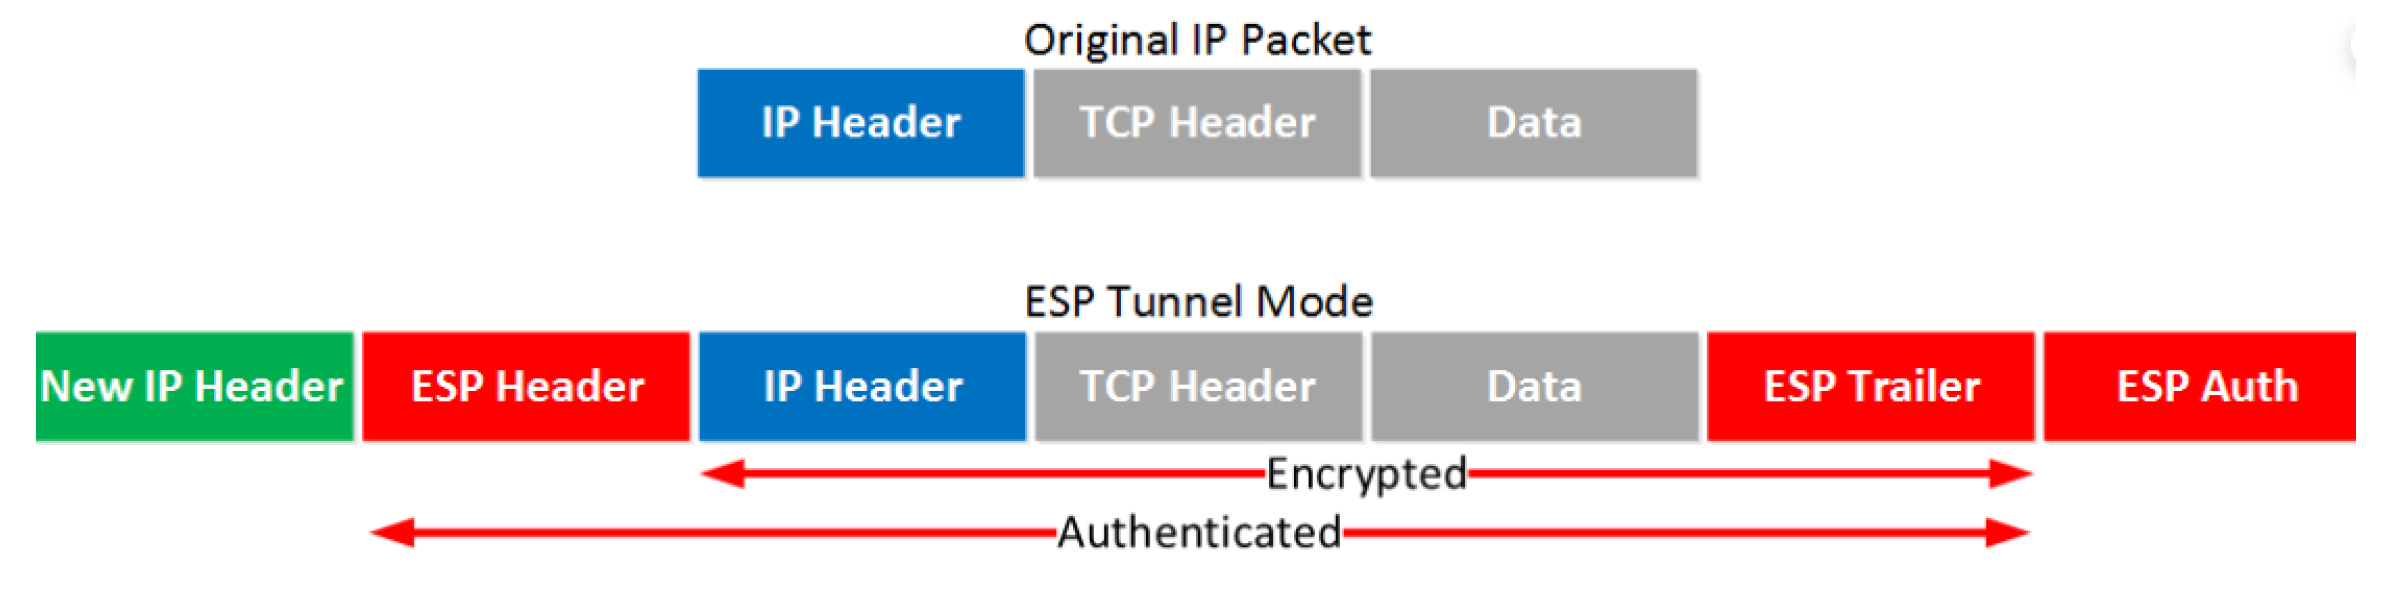
\includegraphics[width=\textwidth]{Images/additionnal_headers_trailers.png}
    \caption{Wireshark capture of the \textit{echo} request through the VPN channel}
    \label{img:IPSec}
\end{figure}

\section{Question - What changes in the routing table after a network link failure ?}

\begin{questionBox}{What changes in the routing table after a network link failure ?}
    Display the routing table of your routers. What have changed ? How much time has it taken to change ? What could happen if you do a ping between PC1 and PC2 before the changes takes place ? What is the current route and its length ? Did the route change and why ?
\end{questionBox}


The usage of a VPN make the content inside of the sent packages unreadable and unchangeable by any malicious actor thanks to the protection (encryption + hash). The big difference between a VPN and a "classical" encrypted channel is that it is the whole packet that is encrypted here. This means that even the emitter/receiver addresses are hidden.
This implies that is used for security reasons, for example when using a public Wi-Fi.\\
It can also be used to bypass firewalls as the destination in the header is just the exit of the VPN channel and not
the real destination of the packet.

\section{Bonus question - VPN Security}

\begin{bonusQuestionBox}{VPN Security}
    Is VPN really a good way to secure your communication ? Why ? If it is not the case, what could you do instead (or in addition) ?
\end{bonusQuestionBox}


The provider of the VPN can still see what you are sending in it and might store/sell this data so you must trust the provider. Once the packets have exited the VPN and are on their way to their real destination, they are no longer protected.\\
A way to prevent it is to encrypt the packets you send through the VPN with an \textit{end to end encryption} (E2EE) such that the content of the packet stays encrypted until the last hop on the network.

\end{document}

% frame.number >= && frame.number <=
